\documentclass[aspectratio=169]{beamer}

\usepackage{graphicx}
\usepackage{amsmath}
\usepackage{xspace}
\usepackage{tikz}
\usepackage{listings}
\usepackage{unicode-math}
\usepackage{environ}
\usepackage{docs/style}
\usepackage{xepersian}

%settings---------------------
\settextfont{Yas}
% Persian specific
\newcommand{\itmsep}[1]{\raggedleft\setlength\itemsep{#1}}
\newcommand{\itemr}{\raggedleft\setlength\itemsep{3mm}}
\newcommand{\fn}[2]{\LR{\LTRfootnote[frame,#1]{~#2}}}
%\newcommand{\fn}[2]{{\LR{\footnote[frame,#1]{{~\LR{#2}}}}}}
\newcommand{\fnn}[1]{{\LR{\footnote[frame]{{~\LR{#1}}}}}}
\newcommand{\m}[1]{\ensuremath{\mathnormal{#1}}}
\newcommand{\mc}[1]{\ensuremath{\mathtt{#1}}}
\newcommand{\scl}{\ensuremath{\Sigma^*}\xspace}
\newcommand{\gcl}{\ensuremath{\Gamma^*}\xspace}
\newcommand{\gin}{\ensuremath{\mathnormal{\in}}\xspace}
%\newcommand{\gand}{\ensuremath{\mathnormal{\land}}\xspace}
\newcommand{\gand}{\&\&\xspace}
\newcommand{\alglr}{\LTR\ttfamily\small}
\newcommand{\st}[1]{\ensuremath{\mathnormal{\{#1\}}}\xspace}
\newcommand{\gst}[1]{\ensuremath{\mathnormal{\{\text{\texttt{#1}}\}}}\xspace}
\newcommand{\cpp}{C++\xspace}
\newcommand{\enc}[1]{\ensuremath{\mathnormal{\langle#1\rangle}}\xspace}
\newcommand{\abo}[1]{\ensuremath{\mathnormal{O(#1)}}\xspace}
\newcommand{\aso}[1]{\ensuremath{\mathnormal{o(#1)}}\xspace}
\newcommand{\aom}[1]{\ensuremath{\mathnormal{\Omega(#1)}}\xspace}
\newcommand{\ath}[1]{\ensuremath{\mathnormal{\Theta(#1)}}\xspace}
\newcommand{\dom}[2]{\ensuremath{\mathnormal{\Big[ \dfrac{#1}{#2} \Big]}}\xspace}

\newcommand{\Proc}[2]{\Statex \textbf{procedure} \textsc{#1}(#2)}
\newcommand{\Func}[2]{\Statex \textbf{function} \textsc{#1}(#2)}
\newcommand{\To}{\textbf{to}\xspace}
\newcommand{\Aand}{\textbf{and}\xspace}
\newcommand{\Aor}{\textbf{or}\xspace}



\newcommand\pro{\ensuremath{\rightarrow}\xspace}
\newcommand\der{\ensuremath{\Rightarrow}\xspace}
\newcommand\ders{\ensuremath{\stackrel{\mbox{*}}{\Rightarrow}}\xspace}
\newcommand{\dern}[1]{\ensuremath{\stackrel{\mbox{\small #1}}{\Rightarrow}}\xspace}
\newcommand\move{\ensuremath{\vdash}\xspace}
\newcommand\moves{\ensuremath{\stackrel{\small *}{\vdash}}\xspace}
\newcommand{\movesn}[1]{\ensuremath{\stackrel{\small *}{\vdash_{#1}}}\xspace}
\newcommand{\moven}[1]{\ensuremath{\mathnormal{\vdash_{#1}}}\xspace}

\newcommand{\code}[1]{{\LR{\texttt{#1}}}}
\newcommand{\txtlr}[1]{\text{\LR{#1}}}


% Abbreviations
\newcommand{\ie}{\latin{i.e.,~}}
\newcommand{\eg}{\latin{e.g.,~}}
\newcommand{\cf}{\latin{cf.~}}
\newcommand{\etal}{\latin{et al.~}}
\newcommand{\etc}{\unskip~\latin{etc.}\xspace}
\newcommand{\apriori}{\latin{a priori}}
\newcommand{\wrt}{\latin{w.r.t.~}}
%\newtheorem{theorem}{Theorem}

\newcommand\NN{\ensuremath{\mathbb{N}}\xspace}
\newcommand\RR{\ensuremath{\mathbb{R}}\xspace}
\newcommand\NNS{\ensuremath{\mathbb{N}^*}\xspace}
\newcommand\NNZ{\ensuremath{\mathbb{N}\backslash\{0\}}\xspace}
\newcommand\RRP{\ensuremath{\mathbb{R}^+}\xspace}
\newcommand\vect[1]{\ensuremath{\boldsymbol{\vec{#1}}}}
\newcommand\MP{\ensuremath{\mathcal{P}}\xspace}

\newcommand\de{\mathrel{\bullet\mkern-2.5mu{\rightarrow}}}
\newcommand\ue{\mathrel{\bullet\mkern-3mu{-}\mkern-3mu\bullet}}

\DeclareMathOperator*{\argmax}{arg\,max}
\DeclareMathOperator*{\argmin}{arg\,min}

\DeclareMathOperator{\lcm}{lcm}
\DeclareMathOperator{\Spec}{Spec}
\DeclareMathOperator{\Res}{Res}
%\DeclareMathOperator{\land}{and}

\newcommand{\fl}[1]{\ensuremath{\lfloor #1 \rfloor}}
\newcommand{\bfl}[1]{\ensuremath{\big\lfloor #1 \big\rfloor}}
\newcommand{\Bfl}[1]{\ensuremath{\Big\lfloor #1 \Big\rfloor}}
\newcommand{\bgfl}[1]{\ensuremath{\bigg\lfloor #1 \bigg\rfloor}}
\newcommand{\Bgfl}[1]{\ensuremath{\Bigg\lfloor #1 \Bigg\rfloor}}

\newcommand{\cl}[1]{\ensuremath{\lceil #1 \rceil}}
\newcommand{\bcl}[1]{\ensuremath{\big\lceil #1 \big\rceil}}
\newcommand{\Bcl}[1]{\ensuremath{\Big\lceil #1 \Big\rceil}}
\newcommand{\bgcl}[1]{\ensuremath{\bigg\lceil #1 \bigg\rceil}}
\newcommand{\Bgcl}[1]{\ensuremath{\Bigg\lceil #1 \Bigg\rceil}}

\newcommand{\mtx}[1]{\begin{pmatrix} #1 \end{pmatrix}}
\newcommand{\smtx}[1]{\begin{psmallmatrix} #1 \end{psmallmatrix}}

\definecolor{commentgreen}{RGB}{2,112,10}
\definecolor{eminence}{RGB}{108,48,130}
\definecolor{brightmaroon}{rgb}{0.76, 0.13, 0.28}
\definecolor{darkred}{rgb}{0.55, 0.0, 0.0}
\lstset {
    language=C++,
    frame=tb,
    tabsize=4,
    showstringspaces=false,
    numbers=left,
    %upquote=true,
    commentstyle=\color{commentgreen},
    keywordstyle=\color{eminence},
    stringstyle=\color{darkred},
    basicstyle=\small\ttfamily, % basic font setting
    emph={int,char,double,float,unsigned,long,short,void,bool},
    emphstyle={\color{blue}},
    %escapechar=\&,
    % keyword highlighting
    %classoffset=1, % starting new class
    %otherkeywords={>,<,.,;,-,!,=,~},
    %morekeywords={>,<,.,;,-,!,=,~},
    %keywordstyle=\color{weborange},
    %classoffset=0,
}

\makeatletter
\NewDocumentCommand{\LeftComment}{s m}{%
	\IfBooleanF{#1}{\hspace*{\ALG@thistlm}}\textcolor{commentgreen}{\(~\triangleright\) #2}}
\makeatother


\newenvironment{itemframe}[2]{
\begin{frame}[environment=itemframe]{#1}

\framesubtitle{\small \color{gray} \quad #2}
\itemize
\itemr

}{
\enditemize
\end{frame}
}

\newcommand{\centerimg}[2][.5]{
    \begin{figure}[h!]
        \centering
        \includegraphics[width=#1\textwidth]{#2}
    \end{figure}
}

\usetikzlibrary{arrows,calc}
\usetikzlibrary{positioning,shapes,chains,fit}


\tikzset{
    %Define style for boxes
    node/.style={
        circle,
        draw=black, thick,
        align=center,
    },
    ss/.style={
        circle,
        draw=black,
        align=center,
    },
    proc/.style={
        rounded corners,
        draw=black,
        align=center,
    },
    ifelse/.style={
	ellipse,
	draw=black,
	align=center,
    },
    cloudy/.style={
	cloud,
	cloud puffs=12,
	cloud ignores aspect,
	align=center,
	draw=black,
    },
    txt/.style={
        draw = none,
        align = center,
        font = \footnotesize,
    },
    coin/.style={
        rectangle,
        minimum height=1mm,
        minimum width=1cm,
        draw=black,
        fill=black!20,
        rounded corners
    },
    towercolor/.style={
        fill=black!80
    },
    towerbase/.style={
        trapezium,
        trapezium angle=75,
        trapezium stretches=true,
        towercolor,
        minimum width=7mm,
        minimum height=2mm,
    },
    tower/.style={
        rectangle,
        rounded corners,
        towercolor,
        minimum width=2mm,
        minimum height=26mm,
    },
    start-end/.style={
        draw,
        rectangle,
        rounded corners,
    },
    input/.style={ % requires library shapes.geometric
        draw,
        trapezium,
        trapezium left angle=60,
        trapezium right angle=120,
    },
    operation/.style={
        draw,
        rectangle
    },
    loop/.style={ % requires library shapes.misc
        draw,
        chamfered rectangle,
        chamfered rectangle xsep=2cm
    },
    decision/.style={ % requires library shapes.geometric
        draw,
        diamond,
        aspect=#1
    },
    decision/.default=1,
    print/.style={ % requires library shapes.symbols
        draw,
        tape,
        tape bend top=none
    },
    connection/.style={
        draw,
        circle,
        radius=5pt,
    },
    process rectangle outer width/.initial=0.15cm,
    predefined process/.style={
        rectangle,
        draw,
        append after command={
        \pgfextra{
          \draw
          ($(\tikzlastnode.north west)-(0,0.5\pgflinewidth)$)--
          ($(\tikzlastnode.north west)-(\pgfkeysvalueof{/tikz/process rectangle outer width},0.5\pgflinewidth)$)--
          ($(\tikzlastnode.south west)+(-\pgfkeysvalueof{/tikz/process rectangle outer width},+0.5\pgflinewidth)$)--
          ($(\tikzlastnode.south west)+(0,0.5\pgflinewidth)$);
          \draw
          ($(\tikzlastnode.north east)-(0,0.5\pgflinewidth)$)--
          ($(\tikzlastnode.north east)+(\pgfkeysvalueof{/tikz/process rectangle outer width},-0.5\pgflinewidth)$)--
          ($(\tikzlastnode.south east)+(\pgfkeysvalueof{/tikz/process rectangle outer width},0.5\pgflinewidth)$)--
          ($(\tikzlastnode.south east)+(0,0.5\pgflinewidth)$);
        }  
        },
        text width=#1,
        align=center
    },
    predefined process/.default=1.75cm,
    man op/.style={ % requires library shapes.geometric
        draw,
        trapezium,
        shape border rotate=180,
        text width=2cm,
        align=center,
    },
    extract/.style={
        draw,
        isosceles triangle,
        isosceles triangle apex angle=60,
        shape border rotate=90
    },
    merge/.style={
        draw,
        isosceles triangle,
        isosceles triangle apex angle=60,
        shape border rotate=-90
    },
}

\setmathfont{Latin Modern Math}

%cover page info--------------
\title{الگوریتم‌های پیشرفته}
\author{آرش شفیعی}
\institute{
\includegraphics[height=1.2cm]{logos/ui.png}}
\date{}

\begin{document}
%cover page-------------------
\begin{frame}[plain]
	\centering{به نام خدا}
	\maketitle
\end{frame}

\setcounter{framenumber}{0}
\raggedleft

%toc---------------------------
\begin{frame}{فهرست مطالب}
\begin{flushright}
	\tableofcontents
\end{flushright}
\end{frame}

%refrences----------------
\begin{frame}{کتاب‌های مرجع}
	\begin{itemize}\itmsep{5mm}
		\item[-]
مقدمه‌ای بر الگوریتم‌ها از کرمن، لایسرسون، ریوست، و استاین
		\fn{1}{Introduction to Algorithms, by Cormen, Leiserson, Rivest, and Stein}
	\end{itemize}
\end{frame}

%chpaters--------------------
\section{الگوریتم‌های پیشرفته در گراف}
%------------------------------------------------------------------------
\begin{frame}{يادآوری}
	\begin{itemize}\itemr
		\item[-]
کتاب CLRS که مرجع اصلی این درس است دو تعریف مجزا برای گراف ارائه می‌دهد:
\item[۱]
گراف بدون جهت: این گراف نمی‌تواند طوقه یا یال موازی داشته باشد.
\item[۲]
گراف جهت دار: این گراف می‌تواند طوقه داشته باشد اما نمی‌تواند یال موازی داشته باشد. البته دو یال می‌تواند بین دو راس یکسان وجود داشته باشد به شرطی جهت آنها مخالف یکدیگر باشد. برای مثال شکل زیر یک گراف فاقد یال موازی است.

\begin{figure}[h!]
\centering
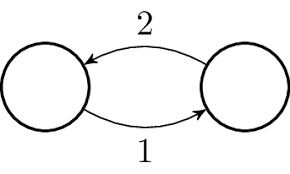
\includegraphics[width=0.2\textwidth]{figs/chap01/1.png}
\end{figure}
\item[-]
در هر یک از مسائل بسته به ذات مسئله نوع خاصی از گراف به عنوان ورودی در نظر گرفته می‌شود. برای مثال ورودی مسئله کوتاه ترین مسیر در حالت کلی یک گراف جهت دار و وزن دار است.
\end{itemize}
\end{frame}


%------------------------------------------------------------------------
\begin{frame}{يادآوری}
	\begin{itemize}\itemr
\item[-]
الگوریتم‌های گراف برخلاف بیشتر الگوریتم‌هایدارای دو متغییر تاثیر گذار در اندازه ورودی‌اند: تعداد یال‌ها (|E|) و تعداد رئوس (|V|) .
\item[-]
بر اساس قرارداد کتاب CLRS می‌توان در نمادهای مجانبی از قرار دادن نماد اندازه در اطراف V و E صرف‌نظر ‌کرد.

\item[-]
الگوریتم‌های گراف به طور معمول در دو حالت بررسی می‌شوند:
\item[الف]
زمانی که گراف متراکم باشد: در این حالت فرض میکنیم همه رئوس به هم متصل هستند بنابراین تعداد یال ها از مرتبه
\ath{V^2}
است.
\item[ب]
زمانی که گراف خلوت باشد:‌ در این حالت به طور معمول فرض می‌شود که تعداد یال‌ها از مرتبه
\ath{V}
است.

	\end{itemize}
\end{frame}

%------------------------------------------------------------------------
\begin{frame}{يادآوری}
\begin{itemize}\itemr
\item[-]
پیچیدگی زمانی ارائه شده برای یک الگوریتم گراف را می‌توان در دو حالت بالا تحلیل کرد. برای مثال تمرین زیر از کتاب CLRS را در نظر بگیرید:

\begin{figure}[h!]
\centering
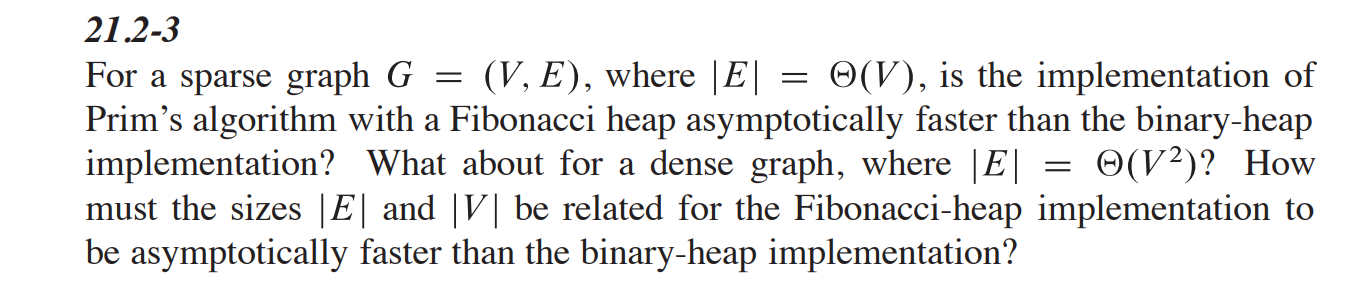
\includegraphics[width=\textwidth]{figs/chap01/2.png}
\end{figure}

\end{itemize}
\end{frame}

%------------------------------------------------------------------------
\begin{frame}{يادآوری}
\begin{itemize}\itemr
\item[-]
پیچیدگی زمانی الگوریتم پریم با استفاده از هرم دودویی از مرتبه
\m{O(E logV+V lgV)}
و با استفاده از هرم فیبوناچی از مرتبه
\m{O(E+V logV)}
است. با جایگذاری V به جای E در این دو تابع درمی‌یابیم که در گراف خلوت هر دو پیاده‌سازی‌ از لحاظ مجانبی سرعت یکسانی دارند و از مرتبه
\m{O(Vlg V)}
اند. اما در گراف متراکم پیاده‌سازی با هرم فیبوناچی از لحاظ مجانبی سریع تر و از مرتبه
\m{O(lgV^2)}
 است.
\item[-]
چنین تحلیلی در دیگر الگوریتم‌‌های گراف هم کاربرد دارد. برای مثال الگوریتم فلوید-وارشال از مرتبه زمانی
\m{O(V^3)}
 است. از تحلیل این تابع می‌توان نتیجه گرفت خلوت یا متراکم بودن گراف از نظر مجانبی تاثیری بر سرعت این الگوریتم ندارد.
\end{itemize}
\end{frame}



 %5 pages
%------------------------------------------------------------------------
\begin{frame}{الگوریتم جانسون}
\begin{itemize}\itemr
\item[-]
الگوریتم جانسون
\fn{1}{Johnson Algorithm}
مانند الگوریتم فلوید وارشال برای یافتن کوتاه ترین مسیر بین هر دو راس گراف است. این الگوریتم برای گراف‌های خلوت پبچیدگی زمانی کمتری نسبت به بقیه روش‌ها (فلوید وارشال و روش شبیه‌سازی ضرب ماترسی) دارد.

\item[-]
الگوریتم جانسون -مانند الگوریتم بلمن فورد- می‌تواند روی گراف دارای یال منفی کوتاه ترین مسیر را به درستی محاسبه کند و وجود دور منفی در گراف را تشخیص و گزارش دهد. (گراف دارای دور منفی در مسئله کوتاه ترین مسیر یک حالت خطا محسوب می‌شود.)
\footnote{برای گراف دارای دور منفی یافتن کوتاه ترین مسیر ساده می‌تواند کاربرد داشته‌باشد. این مسئله ان‌پی-سخت است.}
\end{itemize}
\end{frame}

%------------------------------------------------------------------------
\begin{frame}{الگوریتم جانسون}
	\begin{itemize}\itemr
\item[-]
برای طراحی یک الگوریتم مسئله کوتاه‌ترین مسیر بین هر جفت رأس می‌توان V بار اجرا کردن یکی از الگوریتم‌های کوتاه‌ترین مسیرهای هم مبداء را به عنوان یک حد بالا برای مرتبه زمانی تحلیل کرد.

\item[-]
برای مثال
\m{|V|}
بار اجرای الگوریتم بلمن فورد مرتبه
\m{O(V^2E)}
و
\m{|V|}
بار اجرای الگوریتم دایجسترا مرتبه
\m{O(VE+V^2lgV)}
را به دست می‌دهد.
\item[-]
روش دوم سریع‌تر است امّا در گراف‌‌هایی که یال منفی داشته باشند به درستی کار نمی‌کند.
	\end{itemize}
\end{frame}

%------------------------------------------------------------------------
\begin{frame}{الگوریتم جانسون}
\begin{itemize}\itemr
\item[-]
الگوریتم جانسون نیز از ایده‌ایی مشابه استفاده می‌کند. این الگوریتم هر دو الگوریتم بلمن-فورد و دایجسترا را فراخوانی می‌کند؛
\item[۱]
جانسون در مرحله اول، الگوریتم بلمن-فورد را استفاده می‌کند تا وجود دور منفی را تشخیص دهد و در صورتی که دور منفی وجود داشت آن را گزارش داده و کار تمام می‌شود.
\item[۲]
در صورتی که دور منفی وجود نداشت، این الگوریتم با استفاده از روشی که در ادامه بررسی خواهد شد، همه وزن‌ها را به مقادیر غیر منفی نگاشت می‌کند.
\item[۳]
حال که همه وزن‌‌های غیر منفی شده‌اند برای هر رأس یک بار الگوریتم دایجسترا اجرا می‌شود تا کوتاه ترین مسیرها از هر رأس به بقیه رئوس محاسبه شوند.
\end{itemize}
\end{frame}

%------------------------------------------------------------------------
\begin{frame}{الگوریتم جانسون}
	\begin{itemize}\itemr
\item[-]
اما چطور باید وزن‌های گراف را به مقادیر غیر منفی نگاشت کرد؟ واضح است که بعد از تغییر وزن‌ها نباید کوتاه ترین مسیرها را تغییر کنند. برای مثال اضافه کردن یک مقدار ثابت به همه وزن‌ها نگاشت مناسبی نیست. برای درک بهتر این موضوع به مثال زیر توجه کنید:
\begin{center}
	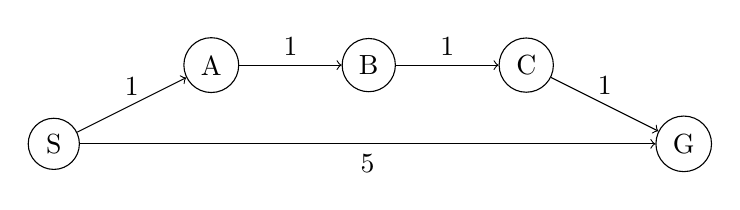
\begin{tikzpicture}[->]
		\node[circle,draw] (S) at (0,0) {S};
		\node[circle,draw] (G) at (8,0) {G};
		\node[circle,draw] (A) at (2,1) {A};
		\node[circle,draw] (B) at (4,1) {B};
		\node[circle,draw] (C) at (6,1) {C};

		\draw (S) -- node[below] {5} (G);
		\draw (S) -- node[above] {1} (A);
		\draw (A) -- node[above] {1} (B);
		\draw (B) -- node[above] {1} (C);
		\draw (C) -- node[above] {1} (G);
	\end{tikzpicture}
\end{center}
\item[-]
اضافه کردن یک واحد به همه یال‌ها کوتاه ترین مسیر از S به G را تغییر می‌دهد:

\begin{center}
	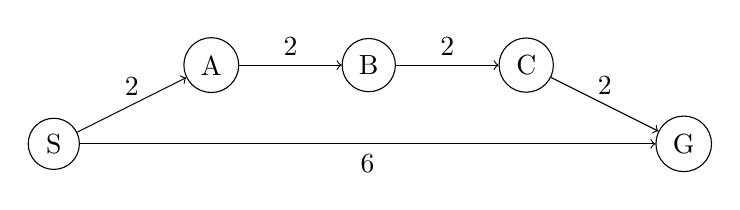
\begin{tikzpicture}[->]
		\node[circle,draw] (S) at (0,0) {S};
		\node[circle,draw] (G) at (8,0) {G};
		\node[circle,draw] (A) at (2,1) {A};
		\node[circle,draw] (B) at (4,1) {B};
		\node[circle,draw] (C) at (6,1) {C};

		\draw (S) -- node[below] {6} (G);
		\draw (S) -- node[above] {2} (A);
		\draw (A) -- node[above] {2} (B);
		\draw (B) -- node[above] {2} (C);
		\draw (C) -- node[above] {2} (G);
	\end{tikzpicture}
\end{center}

	\end{itemize}
\end{frame}

%------------------------------------------------------------------------
\begin{frame}{الگوریتم جانسون}
	\begin{itemize}\itemr
\item[-]
بیایید ویژگی‌های این تغییر وزن را به طور دقیق‌تر بررسی کنیم؛\\
فرض کنید وزن‌های گراف توسط تابعی به نام «تابع وزن»
\fn{1}{weight function}
داده شده. به طوری که وزن یال بین u و v برابر است با
\m{w(u, v)}.
آنگاه تابع وزن جدیدی مانند
\m{\hat{w}}
باید این دو ویژگی را داشته باشد:
\item[1]
به ازای هر
\m{u, v \in E}
مسیری مانند p با استفاده از تابع وزن
\m{w}
یک کوتاه ترین مسیر از u به v است اگر و تنها اگر مسیر p با استفاده از تابع وزن
\m{\hat{w}}
نیز یک کوتاه ترین مسیر باشد.
\item[2]
به ازای هر
\m{u, v \in E}
مقدار
\m{\hat{w}(u, v)}
غیر منفی باشد.
	\end{itemize}
\end{frame}

%------------------------------------------------------------------------
\begin{frame}{الگوریتم جانسون}
	\begin{itemize}\itemr
\item[-]
الگوریتم جانسون از این تغییر وزن استفاده می‌کند:
\begin{align*}
	\m{\hat{w}(u, v)} = \m{w(u, v)} + h(u) - h(v)
\end{align*}
\item[-]
به طوری که u رأس شروع و v رأس پایان یال است و h تابعی است که به هر رأس یک عدد حقیقی نسبت می‌دهد.
\item[-]
در ادامه ثابت خواهیم کرد که این تغییر وزن به ازای هر تابع h کوتاه‌ترین مسیرها را تغییر نمی‌دهد اما برای تبدیل همه وزن‌ها به مقادیر غیر منفی، تابع h باید به درستی تعریف شود.
	\end{itemize}
\end{frame}
%------------------------------------------------------------------------
\begin{frame}{الگوریتم جانسون}
	\begin{itemize}\itemr
		\item[-]
ابتدا باید ثابت ‌کنیم رابطه تغییر وزن ارائه شده ویژگی اول را ارضاء می‌کند.
		\item
فرض کنید
		\m{ p= \langle v_0, v_1, ..., v_k \rangle}
یک مسیر از
		\m{v_0}
به
		\m{v_k}
باشد. همچنین وزن کل مسیر p با تابع وزن w را با  w(p) نشان می‌دهیم. آنگاه
		\m{\hat{w}}
برابر است با:
		\begin{align*}
			\m{\hat{w}(p)= (\hat{w}(v_0, v_1) + h(v_0) -  h(v_1)) + (\hat{w}(v_1, v_2) + h(v_1) -  h(v_2)) + }
			\\
			\m{(\hat{w}(v_2, v_3) + h(v_2) -  h(v_3)) + ... + (\hat{w}(v_{k-1}, v_k) + h(v_{k-1}) -  h(v_k))}
		\end{align*}

	\end{itemize}
\end{frame}
%------------------------------------------------------------------------
\begin{frame}{الگوریتم جانسون}
	\begin{itemize}\itemr
\item
رابطه بالا نشان می‌دهد برای هر رأس مثل u، مقدار h(u) به وزن یک یال اضافه می‌شود و از یال بعدی کسر می‌شود (به غیر از رأس ابتدا و انتهای مسیر). بعد از ساده‌سازی به این رابطه می‌رسیم:
\begin{align*}
	\m{\hat{w}(p)=w(p) + h(h(v_0) - h(v_k)}
\end{align*}
\item
بنابراین برای هر دو رأس مشخص به همه کوتاه‌ترین مسیرهای بین آن دو رأس یک مقدار ثابت اضافه می‌شود پس این نگاشت وزن کوتاه ترین مسیرها را تغییر نمی‌دهد.
	\end{itemize}
\end{frame}

%------------------------------------------------------------------------
\begin{frame}{الگوریتم جانسون}
	\begin{itemize}\itemr
		\item[-]
هدف بعدی این است که شرایطی فراهم کنیم که ویژگی دوم هم برقرار باشد. برای این کار یک رأس جدید به نام s به گراف اضافه می‌کنیم. سپس این رأس را با یال‌هایی با وزن صفر به همه رئوس دیگر متصل می‌کنیم به طوری که یال ‌ها از s خارج شوند.
		\begin{figure}[h!]
			\centering
			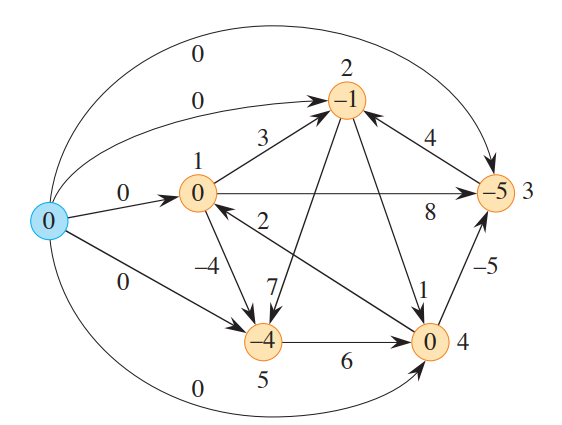
\includegraphics[width=.4\textwidth]{figs/chap02/4.png}
		\end{figure}
شکل بالا نمونه‌ایی از این تغییر را نشان می‌دهد (رأس آبی رنگ به گراف اضافه شده‌است).
	\end{itemize}
\end{frame}

%------------------------------------------------------------------------
\begin{frame}{الگوریتم جانسون}
	\begin{itemize}\itemr
		\item
سپس تعریف می‌کنیم مقدار h برای هر رأس مثل v برابر است با کوتاه ترین مسیر از s به v . در شکل بالا نیز اعداد نوشته‌شده بر رأس‌ها به همین طریق محاسبه شده‌اند.
		\item
حال با استفاده از نامساوی مثلثاتی می‌دانیم که به ازای هر
		\m{(u, v \in E)}
رابطه زیر برقرار است:
		\begin{center}
			\m{h(v) \leqslant h(u)+w(u, v) } \\

		\end{center}
		\item
اگر رابطه بالا برقرار نباشد نتیجه می‌شود که مسیر h(v) کوتاه‌ترین مسیر نبوده و به تناقض می‌رسیم.
		\item
سپس h(u) را به سمت راست نامساوی می‌بریم:
		\begin{center}
			\m{0\leqslant w(u, v) + h(u) - h(v)}
		\end{center}
		\item
سمت راست این نامساوی همان رابطه‌ایی است که برای $\hat{w}$ تعریف شد. بنابراین ثابت شد که به ازای هر
		\m{(u, v \in E)}
مقدار $\hat{w}$ غیر منفی است.
	\end{itemize}
\end{frame}

%------------------------------------------------------------------------
\begin{frame}{الگوریتم جانسون}
	\begin{itemize}\itemr
		\item[-]
درستی الگوریتم جانسون ثابت شد. شکل زیر یک نمونه از گراف تغییر وزن یافته توسط الگوریتم جانسون است:
		\begin{figure}[h!]
			\centering
			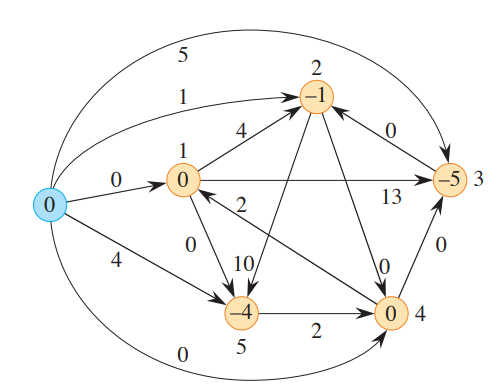
\includegraphics[width=.3\textwidth]{figs/chap02/5.png}
		\end{figure}

		\item[-]
قبلا اشاره شد که الگوریتم جانسون از الگوریتم بلمن-فورد برای تشخیص دور منفی استفاده می‌کند. همچنین دیدم که برای محاسبه تابع h نیاز به مقادیر کوتاه‌ترین مسیر از s به بقیه رئوس نیاز داریم. می‌دانیم الگوریتم بلمن-فورد توانایی محاسبه هر دوی این موارد را دارد. بنابراین الگوریتم جانسون با یک بار اجرای بلمن-فورد هم کوتاه‌ترین مسیرها از s را محاسبه می‌کند و هم وجود دور منفی را تشخیص می‌دهد.

	\end{itemize}
\end{frame}

%------------------------------------------------------------------------
\begin{frame}{الگوریتم جانسون}
	\begin{itemize}\itemr
		\item[-]
		برای یافتن وزن اصلی یک مسیر از رابطه زیر استفاده می‌کنیم:
		\begin{center}
			\m{w(p(u, v)) = \hat{w}(p(u, v)) + h(v) - h(u) }
		\end{center}

		\item[-]
		در نهایت به تحیلی پیچیدگی زمانی الگوریتم جانسون می‌پردازیم:
		\item
		اجرای $|V|$ بار الگوریتم دایجسترا زمان‌برترین مرحله الگوریتم جانسون است بنابراین -مانند دایجسترا- باید گراف را در لیست مجاورتی ذخیره کنیم. حال اگر فرض کنیم الگوریتم دایجسترا با استفاده از هرم فیبوناچی پیاده‌سازی شده‌است، پیچیدگی زمانی برابر است با
		\m{O(V^2lgV+VE)}
		که از ضرب یک
		\m{|V|}
		در مرتبه زمانی دایجسترا به دست آمده‌است.
		\item
		در صورتی که گراف خلوت باشد مرتبه زمانی این الگوریتم برابر است
		\m{O(V^2lgV)}.
		در حالی که الگوریتم فلوید-وارشال برای گراف خلوت از مربته زمانی
		\m{O(V^3)}
		است.

	\end{itemize}
\end{frame} %12 pages
%------------------------------------------------------------------------
\begin{itemframe}{مسئله شار بیشینه}{معرفی مسئله}
\item [-]
در دنیای واقعی شبکه‌های بسیاری وجود دارند که با هدف انتقال چیزی ساخته شده‌اند. برای مثال شبکه‌های آب رسانی، مدارات الکتریکی(انتقال جریان الکتریکی)، خطوط راه‌آهن و غیره. به طور معمول در چنین شبکه‌هایی افزایش نرخ انتقال مطلوب است. بنابراین مسئله شار بیشینه می‌پرسد‌: چگونه می‌توان نرخ انتقال را در این شبکه‌ها بیشینه کرد؟
\item [-]
برای حل یک مسئله شار بیشینه باید شبکه را توسط گراف مدلسازی کرد. به این گراف «شبکه شار»
\fn{1}{flow network}
و به هر چیزی که در این شبکه در جریان باشد به طور کلی شار
\fn{2}{flow}
 گفته می‌شود.
\end{itemframe}

%------------------------------------------------------------------------
\begin{itemframe}{مسئله شار بیشینه}{معرفی مسئله}
	\item [-]
برای درک بهتر مسئله شار بییشیه ويژگی‌های این مسئله را همراه با مثال شبکه آب رسانی توضیح می‌دهیم؛
	\item
در مسئله شار بیشیه گراف ثابت فرض می‌شود. (مثال: خطوط آب‌رسانی مثل لوله‌ها و اتصالات از قبل ساخته شده‌ و غیر قابل تغییر اند.)
	\item
هر یال یک ظرفیت مشخص برای انتقال شار دارد و نمی‌تواند بیشتر از آن مقدار انتقال دهد. (مثال: هر لوله آب -بسته به قطر لوله‌- می‌تواند مقدار آبی مشخصی را از خود عبور دهد.)
	\item
سرعت انتقال شار در سراسر شبکه ثابت فرض می‌شود. (مثال: نمی‌توانیم تعیین کنیم آب با فشار بیشتری وارد لوله‌ها شود بنابراین سرعت حرکت آب در لوله‌ها یکسان است.)
\end{itemframe}

%------------------------------------------------------------------------
\begin{itemframe}{مسئله شار بیشینه}{معرفی مسئله}

	\item
در مسئله شار بیشینه تنها متغییری که ما می‌توانیم تعیین کنیم این است که چقدر از ظرفیت هر یال برای انتقال شار استفاده کنیم. (مثال: می‌توانیم یک شیر آب سر راه هر لوله قرار دهیم و بعد از حل مسئله شار بیشینه تعیین کنیم هر شیر اجازه ورود چه حجمی از آب را بدهد.)
	\item
مجموع شار ورودی به هر رأس باید با مجموع شار خروجی برابر باشد. به عبارت دیگر هیچ شاری نمی‌تواند در رأس‌های گراف ذخیره شود یا از بین برود. به این قانون، قانون بقای شار
\fn{1}{flow conservation}
گفته می‌شود.
(مثال: بدیهیست در اتصالاتی که لوله‌ها را به هم وصل می‌کند آب نمی‌تواند ذخیره شود یا نشت کند. ممکن هر اتصال یک یا چند لوله ورودی و خروجی داشته باشد در هر صورت مجموع آب ورودی و خروجی باید برابر باشد.)

\end{itemframe}

%------------------------------------------------------------------------
\begin{itemframe}{مسئله شار بیشینه}{معرفی مسئله}

	\item[-]
با این توضیحات شاید به نظر برسد که برای حل این مسئله کافیست به طور حریصانه از همه ظرفیت همه یال‌ها برای انتقال استفاده کنیم. (مثال: همه شیر آب‌هایی که سر راه لوله‌ها قرار گرفته اند را تا بیشترین مقدار باز کنیم تا در صورتی که مقدار کافی آب به آن لوله رسید از تمام ظرفیت آن لوله برای انتقال آب استفاده کنیم.)
	\item[-]
نکته جالب اینجاست که برخلاف انتظار این الگوریتم حریصانه جواب بهنیه را تولید نمی‌کند. در ادامه مثال‌هایی خواهیم دید که ممکن است کاهش مقدار شار گذرنده از یک یال باعث افزایش شار کلی گذرنده از شبکه شود. (مثال: در شبکه آب رسانی ممکن است با بستن شیر، اجازه ورود حجم کمتری از آب به یک لوله را بدهیم و با این کار شار گذرنده از شبکه را بیشتر کنیم.)
\end{itemframe}

%------------------------------------------------------------------------
\begin{itemframe}{مسئله شار بیشینه}{تعاریف رسمی}
\item[-]
قبل ادامه بحث بهتر است با یک تعریف دقیق و رسمی از شبکه شار آشنا شویم؛
\item
شبکه شار یک گراف جهت‌دار است. به این معنی که شار نمی‌تواند در یک یال در دو جهت حرکت کند.

شبکه شار همرا با تابع c به ورودی مسئله داده می‌شود. تابع c یال‌ها و ظرفیت‌‌ها را نگاشت می‌کند به طوری که ظرفیت یال u به v برابر است با
\m{c(u, v)} .
\item
شبکه شار دارای دو رأس خاص است که ورود شار به شبکه (و یا تولید شار) و خروج از شار شبکه (و یا مصرف شار) را مدل می‌کنند. به این دو رأس منبع
\fn{1}{source}
و مقصد
\fn{2}{sink}
گفته می‌شود. به طور معمول به رأس منبع با s و رأس مقصد با t نشان داده می‌شوند.
\item
رأس منبع و مقصد تنها رئوسی هستند که از قانون بقای شار پیروی نمیکنند.
\end{itemframe}

%------------------------------------------------------------------------
\begin{itemframe}{مسئله شار بیشینه}{تعاریف رسمی}
\item
همانطور که قبلا اشاره شد، گراف جهت‌دار می‌تواند طوقه داشته‌باشد. امّا وجود طوقه در شبکه شار غیر مجاز است.
\item
همچنین دیدیم که وجود یال‌های پادموازی نیز در گراف جهت‌دار بلامانع است. امّا در شبکه شار یال‌های پادموازی هم غیر مجاز اند.(در بخش يادآوری فصل یال‌های پادموازی بحث شده‌اند.)
\item
حذف طوقه (دور به طول ۱) و یال‌های پادموازی (دور به طول ۲) از پیچیدگی مسئله می‌کاهد.
\item
وجود دورهایی با طول بالا تر در شبکه شار مجاز است.
\end{itemframe}

%------------------------------------------------------------------------
\begin{itemframe}{مسئله شار بیشینه}{تعاریف رسمی}

\item[-]
همچنین باید یک تعریف کمی برای شار کل شبکه ارائه کنیم تا مشخص شود منظور از شار بیشینه چیست؛
\item
خروجی این مسئله کردن تابع f است که یال‌ها را به شار گذرنده از آنها نگاشت می‌کند. به این صورت که شار گذرنده از یال u به v برابر است با
\m{f(u, v)} .

\item
تابع f باید دو ويژگی داشته باشد؛ قانون بقای شار را نقض نکند و از مقدار ظرفیت هر یال تجاوز نکند. در صورتی که تابعی مانند
\m{f'}
این ویژگی‌ها را نقض کند یک تابع شار نیست.

\end{itemframe}

%------------------------------------------------------------------------
\begin{itemframe}{مسئله شار بیشینه}{تعاریف رسمی}
\item
مقدار شار کل شبکه با |f| نشان داده می‌شود و به این صورت تعریف می‌شود: \\
\begin{center}
\m{|f| = \sum_{v \in V} f(s, v) - \sum_{v \in V} f(v, s)}
\end{center}
\item
به زبان ساده این عبارت مجموع شار خالص خروجی از رأس منبع را مشخص می‌کند :مجموع شار خارج شونده از منبع منهای مجموع شار وارد شونده به منبع. (معمولاً مجموع شار وارد شونده به منبع صفر است.)
\item
قرارداد می‌کنیم که اگر بین u و v یال وجود نداشته باشد
\m{f(u, v)}
برابر صفر است.
\end{itemframe}
%------------------------------------------------------------------------
\begin{itemframe}{مسئله شار بیشینه}{تعاریف رسمی}
\item[-]
امّا چطور این کمیّت می‌تواند نماینده شار گذرنده از کل شبکه باشد؟
\item
برای درک بهتر این موضوع به شبکه شار به چشم یک بلوک بزرگ نگاه کنید که از رأس منبع شار به آن وارد و از مقصد خارج می‌شود.
\centerimg[.5]{figs/graph/6.png}

\item
با توجه به قانون بقای شار، شار نمی‌تواند در این بلوک بزرگ بماند بنابراین با همان نرخی که وارد آن می‌شود باید از آن خارج شود. (فرض کنید پیکان‌ها شار خالص را نشان می‌دهند.)‌
\item
بنابراین نرخ خالص شار خروجی از منبع نماینده شاری است که در کل شبکه جریان دارد.
\end{itemframe}


%------------------------------------------------------------------------
\begin{itemframe}{مسئله شار بیشینه}{ساده‌سازی مسئله شار بیشینه}
\item[-]
شاید دقت کرده باشید که در تعریف شبکه شار فرض‌های ساده کننده‌ایی درنظر گرفتیم که لزوماً در یک مسئله واقعی بیشینه‌سازی شار، برقرار نیستند. دو فرض به این شکل داشتیم که در زیر آورده شده‌اند؛
\item[۱]
ممکن است در یک مسئله واقعی بیشینه‌سازی شار چند منبع و چند مقصد داشته باشیم. در حالی که در تعریف شبکه شار تنها یک منبع و مقصد برای شبکه لحاظ کردیم.
\item[۲]
ممکن است در یک مسئله واقعی بیشینه‌سازی شار یال موازی داشته باشیم. درحالی که وجود چنین یالی را در شبکه شار غیر مجاز دانستیم.
\end{itemframe}

%------------------------------------------------------------------------
\begin{itemframe}{مسئله شار بیشینه}{ساده‌سازی مسئله شار بیشینه}
\item[-]
در ادامه نشان می‌دهیم که چطور یک مسئله واقعی بیشینه‌سازی شار را که دارای چند منبع و مقصد است و یال پادمتقارن دارد را مدل کنیم.

\end{itemframe}

%------------------------------------------------------------------------
\begin{itemframe}{مسئله شار بیشینه}{ساده‌سازی مسئله شار بیشینه}
\item
شکل زیر نشان می‌دهد چطور یک شبکه شار با چندین رأس منبع و مقصد را می‌توان به یک شبکه شار با یک منبع و مقصد تبدیل کرد.
\centerimg[.8]{figs/graph/7.png}

\end{itemframe}

%------------------------------------------------------------------------
\begin{itemframe}{مسئله شار بیشینه}{ساده‌سازی مسئله شار بیشینه}
\item
شکل زیر نشان می‌دهد چطور یک شبکه دارای یال‌های پادمتقارن را می‌توان به یک شبکه شار قابل‌قبول تبدیل کرد.
\centerimg[.9]{figs/graph/8.png}
\end{itemframe}
%------------------------------------------------------------------------
\begin{itemframe}{مسئله شار بیشینه}{مثالی از مسئله شار بیشینه}
\item[-]
شکل زیر یک شبکه شار را به همراه شار موجود در آن نشان می‌دهد:
\centerimg[.5]{figs/graph/8-1.png}

\item[-]
برای نشان دادن شبکه شار یک قرارداد شناخته شده وجود دارد که در شکل بالا قابل مشاهده است. به این صورت که ابتدا مقدار شار و سپس ظرفیت هر یال نوشته می‌شود و این دو عدد به وسیله خط مورب از هم جدا می‌شوند.
\end{itemframe}

%------------------------------------------------------------------------
\begin{itemframe}{مسئله شار بیشینه}{مثالی از مسئله شار بیشینه}
\item[-]
همچنین دقت کنید که چگونه قانون پایستگی شار در این شکل رعایت شده. برای مثال ۱۱ واحد به راس
\m{v_4}
وارد شده و ۴ و ۷ واحد از آن خارج می‌شوند.
\item[-]
برای درک مسئله شار بیشینه بهتر است سعی کنیم مسئله را صورت دستی حل کنیم.
\item[-]
برای مثال چطور می‌توان مقدار شار شبکه بالا را افزایش داد؟ به عبارت دیگر باید مقدار شار خروجی از رأس s را بیشتر کنید بدون اینکه قانون پایستگی شار نقض شود. (مقدار شار فعلی ۱۹ واحد است.)
\item[-]
اگر موفق به افزایش شار شبکه شدید چطور می‌توان دریافت که این شار بیشینه است یا خیر؟

\end{itemframe}

%------------------------------------------------------------------------
\begin{itemframe}{مسئله شار بیشینه}{مثالی از مسئله شار بیشینه}
\item[-]
شکل زیر با تغییر مقدار شار ۳ یال، مقدار شار شبکه را به ۲۳ واحد افزایش داده‌است. این سه یال عبارت اند از:
\m{(s, v_2), (v_3, v_2), (v_3, t)}
\centerimg[.5]{figs/graph/8-2.png}

\item[-]
نکته جالب توجه اینجاست که با صفر کردن شار یال
\m{(v_3, v_2)}
موفق به افزایش شار کل شبکه شدیم.
\end{itemframe} %16 pages
%------------------------------------------------------------------------
\begin{itemframe}{مسئله شار بیشینه}{آشنایی با روش فورد-فولکرسون}
\item[-]
روش فورد-فولکرسون
\fn{1}{Ford-Fulkerson method}
برای حل مسئله شار بیشینه طراحی شده‌است. بهتر است که به فورد-فولکرسون «الگوریتم» گفته نشود زیرا پیاده‌سازی دقیقی را مشخص نمی‌کند. بلکه یک چارچوب کلی برای حل مسئله شار بیشینه ارائه می‌دهد و چند پیاده‌سازی مختلف با زمان‌های اجرای متفاوت دارد.
\item[-]
در این بخش ابتدا نحوه کار روش فورد-فولکرسون را بررسی می‌کنیم و در بخش آینده درستی این روش را اثبات می‌کنیم.
\end{itemframe}

%------------------------------------------------------------------------
\begin{itemframe}{مسئله شار بیشینه}{آشنایی با روش فورد-فولکرسون}
\item[-]
مبنای روش فورد-فولکرسون استفاده از یک گراف کمکی به نام گراف متمم
\fn{1}{residual networks}
 است. گراف متمم بسیار شبیه به شبکه شار اصلی است. رأس‌های این گراف همان رأس‌های شبکه شار است امّا یال‌های آن متفاوت است. «ظرفیت یال‌های این گراف نشان می‌دهند که شار در یال های شبکه اصلی چطور می‌تواند تغییر کند.»
\item[-]
گراف متمم برخلاف شبکه شار می‌تواند یال پادمتقارن داشته باشد. امّا تفاوت‌های این دو فقط در همین مسئله است. گراف متتم نیز یک گراف جهت‌دار و دارای دو رأس s و t است. همچنین برای این گراف شار تعریف می‌شود و هر یال ظرفیت مشخصی دارد.
\end{itemframe}
%------------------------------------------------------------------------
\begin{itemframe}{مسئله شار بیشینه}{آشنایی با روش فورد-فولکرسون}
\item[-]
همانطور که گفته‌شد، ظرفیت‌های گراف متمم نشان می‌دهند شار در گراف اصلی چطور می‌تواند تغییر کند. برای مثال به شکل زیر دقت کنید. شکل a یک یال در شبکه شار و شکل b معادل همان یال در گراف متمم است.
\centerimg[.7]{figs/chap01/9.png}
\item[-]
همانطور که مشاهده می‌کنید گراف متمم می‌تواند شامل یالی باشد که در گراف اصلی وجود ندارد.
\item[-]
ظرفیت یال موافق در گراف متمم نشان می‌دهد که ۴ واحد شار می‌توان به یال متناظر در گراف اصلی اضافه کرد. همچنین ظرفیت یال مخالف در گراف متمم نشان می‌دهد که ۶ واحد شار می‌توان از یال متناظر در گراف اصلی کم کرد.
\end{itemframe}

%------------------------------------------------------------------------
\begin{itemframe}{مسئله شار بیشینه}{آشنایی با روش فورد-فولکرسون}
\item[-]
امّا شار در گراف متمم به چه معنیست؟ در روش فورد-فولکرسون شاری که برای گراف متمم قرار می‌دهیم درواقع همان تغییراتی است که می‌خواهیم بر روی شبکه اصلی ایجاد کنیم.
\item[-]
 برای مثال در شکل بالا با اعمال تغییراتی که گراف متمم پیشنهاد می‌دهد یک واحد به شار یال
\m{(u, v)}
 در شبکه اصلی اضافه می‌شود. زیرا در گراف متمم ۲ واحد شار در جهت موافق و ۱ واحد در جهت مخالف داریم.
\item[-]
در اینجا صرفاً برای درک بهتر فقط قسمتی از گراف آورده‌شده. امّا تنها عملیات تعریف شده برای اعمال تغییرات گراف متمم روی شبکه شار، اعمال \textbf{کل} شار گراف متمم بر \textbf{کل} شار اصلی است.
\item[-]
دقت کنید یال پادمتقارن در شبکه شار وجود ندارد بنابراین تبدیل به گراف متمم همیشه ممکن است. در بخش آینده نحوه ساخت گراف متمم را به طور دقیق خواهیم دید. در اینجا هدف ایجاد شهود از نحوه کار گراف متمم است.
\end{itemframe}

%------------------------------------------------------------------------
\begin{itemframe}{مسئله شار بیشینه}{آشنایی با روش فورد-فولکرسون}
\item[-]
بر روی گراف متمم به هر مسیر ساده از منبع تا مقصد «مسیر افزایشی»
\fn{1}{augmenting path}
گفته می‌شود.
\item[-]
مسیر‌های افزایشی ویژگی‌های جالب توجهی دارند:
\item[1]
اگر در گراف متمم یک مسیر افزایشی داشته باشیم و مقداری شار برای این مسیر در نظر بگیریم و شار بقیه گراف را صفر کنیم، در این صورت اعمال تغییرات گراف متمم روی شبکه اصلی باعث افزایش شار می‌شود.
\item[2]
ثابت می‌شود که اگر گراف متمم مسیر افزایشی نداشته باشد، شار گراف اصلی بیشینه است و به جواب رسیده‌ایم.
\end{itemframe}


%------------------------------------------------------------------------
\begin{itemframe}{مسئله شار بیشینه}{آشنایی با روش فورد-فولکرسون}
\item[-]
حال که با گراف متمم آشنا شدیم فهم روش فورد-فولکرسون آسان است. این روش ابتدا کل شار شبکه اصلی را برابر صفر قرار می‌دهد سپس به صورت تکراری اقدام به بهبود مقدار شار می‌کند. مراحل روش فورد-فولکرسون به این ترتیب است:
\item[۱]
شار همه یال‌های شبکه شار را برابر صفر قرار می‌دهیم.
\item[۲]
گراف متمم متناظر با شبکه شار را تشکیل می‌دهیم. درصورتی که مسیر افزایشی وجود نداشته‌باشد، شار بیشینه یافت شده بنابراین کار تمام است.
\item[۳]
درغیر این صورت یک مسیر افزایشی می‌یابیم و بیشترین شار ممکن را برای یال‌های عضو این مسیر در نظر می‌گیریم. و شار بقیه یال‌های گراف متمم را صفر می‌کنیم.
\item[۴]
شار گراف متمم را بر شبکه اصلی می‌افزاییم. و به مرحله ۲ بازمی‌گردیم.

\end{itemframe}

%------------------------------------------------------------------------
\begin{itemframe}{مسئله شار بیشینه}{آشنایی با روش فورد-فولکرسون}
\item[-]
شکل زیر به خوبی نحوه کار روش فورد-فولکرسون را نشان می‌دهد:
\centerimg[.9]{figs/chap01/10.png}
\item[-]
قسمت a نشان دهنده شبکه شار و b نشان دهنده گراف متمم است. و مسیر آبی رنگ یک مسیر افزایشی است.
\item[-]
در این شکل b شار یال‌ها نشان داده نشده و تنها ظرفیت‌ها نشان داده شده‌اند. امّا طبق فورد-فولکرسون می‌دانیم این مقدار در کل گراف صفر و در تمام یال‌های مسیر آبی رنگ ۴ است که بیشترین شار ممکن در این مسیر است. (چرا؟)
\item[-]
بنابراین مقدار |f| در شبکه شار برابر ۱۹ واحد و در گراف متمم برابر ۴ واحد است.
\end{itemframe}

%------------------------------------------------------------------------
\begin{itemframe}{مسئله شار بیشینه}{آشنایی با روش فورد-فولکرسون}
\item[-]
بیایید شار گراف متمم را بر شبکه اعمال کنیم:
\centerimg[.7]{figs/chap01/11.png}
\item[-]
به یال s

\end{itemframe}

%------------------------------------------------------------------------
\begin{itemframe}{مسئله شار بیشینه}{اثبات روش فورد-فولکرسون}
\item[-]
با نحوه کار روش فورد-فولکرسون آشنا شدیم. امّا چرا این روش به درستی کار می‌کند؟
\item[-]
در این بخش اثبات درستی این روش را خواهیم دید. برای اثبات‌ها نیاز است مفاهیمی که در بخش قبل با آنها آشنا شدیم را به طور رسمی به زبان ریاضی تعریف کنیم.
\end{itemframe}

%------------------------------------------------------------------------
\begin{itemframe}{مسئله شار بیشینه}{اثبات روش فورد-فولکرسون}
\item[-]
تعریف رسمی گراف متمم:
\item
در تعریف شبکه شار گفتیم f تابعیست که شار یال‌ها را بازمی‌گرداند. برای شبکه شار G با تابع ظرفیت c و یک شار مانند f بر روی این شبکه، گراف متمم را با
\m{G_f}
و شار آن را با
\m{f'}
 نشان می‌دهیم.
\item
 دقت کنید که f جزئی از تعریف G نیست و یک شبکه شار می‌تواند f های مختلفی داشته باشد. بنابراین این نحوه نوشتار (
\m{G_f}
) مشخص می‌کند گراف متمم متناظر با کدام شبکه و کدام شار از شبکه است.
\end{itemframe}

%------------------------------------------------------------------------
\begin{itemframe}{مسئله شار بیشینه}{اثبات روش فورد-فولکرسون}
\item
تابع ظرفیت گراف متمم به این صورت تعریف می‌شود:
\begin{mnum}
c_f(u, v)=
\begin{cases}
c(u, v)-f(u, v)& \text{if} (u, v) \in E\\

f(v, u)& \text{if} (v, u) \in E\\
0 &\text{otherwise}
\end{cases}
\end{mnum}

\item
تعریف می‌کنیم مقدار تابع c برای یال‌هایی که در گراف وجود ندارند صفر است(پیش از این اشاره کردیم که تابع f نیز همین ویژگی را دارد). این مسئله برای فهم فرمول بالا ضروری است. برای درک بهتر فرمول بالا را در حالت‌های حدی بررسی کنید.(از ظرفیت یال کاملاً استفاده شود، شار یک یال دارای ظرفیت صفر باشد، بین دو رأس یالی وجود نداشته باشد)

\end{itemframe}

%------------------------------------------------------------------------
\begin{itemframe}{مسئله شار بیشینه}{اثبات روش فورد-فولکرسون}
\item[-]
تعریف افزایش شار:
\item
به اعمال تغییرات گراف متمم بر شبکه شار augmentation گفته می‌شود. در ترجمه فارسی از کلمه «افزایش» استفاده می‌کنیم هرچند منظور از این ترجمه، افزایش شار نیست بلکه افزودن شار گراف متمم بر شارِ شبکه شار است.
\item
افزودن شار f به
\m{f'}
را با
\m{f \uparrow f'}
نشان می‌دهیم. و به این صورت تعریف میکنیم:
\begin{mnum}
f \uparrow f'(u, v)=
\begin{cases}
f(u, v)+f'(u, v)-f'(v, u)& \text{if} (u, v) \in E\\
0 &\text{otherwise}
\end{cases}
\label{aug-flow-def}
\end{mnum}
\end{itemframe}

%------------------------------------------------------------------------
\begin{itemframe}{مسئله شار بیشینه}{اثبات روش فورد-فولکرسون}
\item[-]
\m{f \uparrow f'}
نیز یک تابع است که به هر جفت رأس یک مقدار نسبت می‌دهد. ادعا می‌کنیم که این تابع نیز تابع شار است و می‌توانیم آن را جایگزین f کنیم. برای اثبات این ادعا باید ثابت کنیم
\m{f \uparrow f'}
ویژگی‌های تابع شار را دارد. تابع شار تابعی است که به هر جفت رأس یک مقدار نسبت می‌دهد و:
\item[1]
از ظرفیت‌های شبکه شار تجاوز نمی‌کند.
\item[2]
از قانون پایستگی شار پیروی می‌کند.
\item
بنابراین باید بررسی آیا
\m{f \uparrow f'}
این دو ویژگی را دارد یا خیر.
\end{itemframe}

%------------------------------------------------------------------------
\begin{itemframe}{مسئله شار بیشینه}{اثبات روش فورد-فولکرسون}
\item[-]
ویژگی اول به سادگی با توجه به فرمول‌های ۱ و ۲ اثبات می‌شوند. به فرمول ۱ دقت کنید‍؛ شار ظرفیت موافق به دقیقا برابر با تفاضل شار فعلی و حداکثر ظرفیت تعریف می‌شود بنابراین حتی اگر از تمام ظرفیت یال موافق در گراف متمم استفاده کنیم، شار
\m{f \uparrow f'}
از حداکثر نفوذ نمی‌کند.
\item
به دلایل مشابه و با توجه به تعاریف می‌توان اثبات کرد که شار
\m{f \uparrow f'}
از صفر کمتر نمی‌شود.
\end{itemframe}
%------------------------------------------------------------------------
\begin{itemframe}{مسئله شار بیشینه}{اثبات روش فورد-فولکرسون}
\item[-]
برای اثبات ویژگی دوم (پایستگی شار) ابتدا باید ثابت کنیم این رابطه برای هر u برقرار است:

\begin{align}
\sum_{v\in V} f \uparrow f'(u, v)  & - \sum_{v\in V} f \uparrow f'(v, u) \notag \\
&=
 \sum_{v\in V} f(u, v) - \sum_{v\in V} f (v, u)
+
\sum_{v\in V} f'(u, v) - \sum_{v\in V} f'(v, u)
\label{cons}
\end{align}
\item

به زبان ساده این رابطه می‌گوید به ازای هر رأس مثل u\\
تفاضل شار وارد و خارج شونده به u در
\m{ f \uparrow f'} \\
=\\
تفاضل شار وارد و خارج شونده به u در
\m{f} \\
+\\
تفاضل شار وارد و خارج شونده به u در
\m{f'}\\


\end{itemframe}
%------------------------------------------------------------------------
\begin{itemframe}{مسئله شار بیشینه}{اثبات روش فورد-فولکرسون}
\item
در اینجا تساوی \ref{cons} را اثبات نمی‌کنیم. با اعمال رابطه \ref{aug-flow-def} به سمت چپ تساوی این اثبات قابل انجام است. امّا درستی این رابطه به صورت شهودی نیز قابل فهم است؛
\\
شار گراف متمم به همه یال‌ها افزوده شده بنابراین انتظار داریم مقدار شار ورودی به هر رأس، به اندازه شار ورودی به همان رأس در
\m{f'}
افزایش داشته‌باشد. این مسئله برای مجموع شار خروجی نیز صادق است.
\item
اگر به سمت راست این تساوی دقت کنید برابر صفر است زیرا پایستگی در هر دو شار
\m{f}
و
\m{f'}
برقرار است. بنابراین در هر دو شار وارد شونده به یک رأس با شار خارج شونده از آن برابر است.
\end{itemframe}
%------------------------------------------------------------------------
\begin{itemframe}{مسئله شار بیشینه}{اثبات روش فورد-فولکرسون}
\item
حال اگر سمت راست \eq{cons} را صفر بگذاریم نتیجه می‌گیریم:
\begin{align*}
\sum_{v\in V} f \uparrow f'(u, v)  = \sum_{v\in V} f \uparrow f'(v, u)
\end{align*}

\item
بنابراین پایستگی شار در
\m{ f \uparrow f'}
برقرار است. توجه کنید که
\m{f}
و
\m{f'}
هر دو قانون پایستگی شار را رعایت می‌کنند بنابراین قابل انتظار است که شار حاصل افزودن این دو شار نیز چنین باشد.
\end{itemframe}
%------------------------------------------------------------------------
\begin{itemframe}{مسئله شار بیشینه}{اثبات روش فورد-فولکرسون}
\item [-]
تا اینجا ثابت کردیم
\m{ f \uparrow f'}
یک تابع شار است پس قابلیت اعمال بر شبکه شار را دارد، امّا این کافی نیست. می‌خواهیم انجام این کار باعث افزایش مقدار
\m{|f|}
شود. به عبارت دیگر
\m{|f \uparrow f'|}
بزرگ‌تر از
\m{|f|}
باشد.
\item
خواهیم دید که اگر
\m{f'}
به این صورت تعریف شود، این اتفاق همیشه می‌افتد:

\item
به طوری که p یک مسیر افزایشی در گراف متمم است.
\end{itemframe}
%------------------------------------------------------------------------


%overall = 68
\end{document}
